% !TeX program = LuaLaTeX
% !TeX encoding = UTF-8
% !TeX spellcheck = pt_PT
% !TeX hyphenation = pt_PT

% Latex style for final reports and dissertations (Instituto Politécnico de Beja)
% Version 0.8.1, 2021/10/01
% Author: João Paulo Barros, joao.barros@ipbeja.pt
% Com contribuições de Henrique Água-Doce, Nuno Mourinho e Raul Carvalho.

%para texto em Português verdadeiro (pt_PT)
\documentclass[PT]{ipbeja-format}
%for text in real English (also change the magic comment locale to en_GB)
%\documentclass[]{ipbeja-format}

% !TeX program = LuaLaTeX
% !TeX encoding = UTF-8
% !TeX spellcheck = pt_PT
% !TeX hyphenation = pt_PT

% Para preencher
\newcommand{\ESCOLA}{Escola Superior de Tecnologia e Gestão}
\newcommand{\CURSO}{Licenciatura em Engenharia Informática}

\newcommand{\TITULO}{Relatório de Estágio}
\newcommand{\SUBTITULO}{Desenvolvimento em Backend na Optiply}

\newcommand{\NOMEALUNO}{Gonçalo Candeias Amaro}
\newcommand{\LOCAL}{Beja, Portugal}

\newcommand{\ORIENTADORIPBEJAA}{Gonçalo Fontes}
% se existir segundo orientador do IPBeja, retirar o comentário da linha seguinte
%\newcommand{\ORIENTADORIPBEJAB}{Colocar o nome do(a) segundo(a) docente orientador(a), se existente}

%se for um estágio deve ser retirado o comentário da linha seguinte e indicar o orientador na entidade de acolhimento do estágio
\newcommand{\ORIENTADORENTIDADE}{Fábio Belga}

%Completar e comentar um dos seguintes dois \newcommand
%\newcommand{\DECLARACAOPROJETO}{Relatório de projeto de fim de curso apresentado na\linebreak \ESCOLA{} do Instituto Politécnico de Beja}
\newcommand{\DECLARACAO}{Relatório de estágio, realizado na Optiply, apresentado na\linebreak \ESCOLA{} do Instituto Politécnico de Beja}

% retirar comentário e preencher se existente
%\newcommand{\DEDICATORIA}{ texto a colocar }
%LOL! NOPE, NIGGA. Do you want me to act like Snoop Dogg in the Hollywood star award? "I wanna thank me for believing in me."

\usepackage[]{hyperref}
\hypersetup{hidelinks,hypertexnames=true}

\begin{document}
\pagenumbering{roman}
\setcounter{page}{1}
\folhacapa % 2.1 das normas
\folharosto % 2.3 das normas
%%%%%%%%%%%%%%%%%%%%%%%%%%%%%%%%%%%%%%%%%%%%
\frontmatter % parte inicial

\clearpage
\chapter{Resumo}
\section*{\textit{\TITULO}\\  {\small{\textit{\SUBTITULO}}}}

\textit{Este relatório consiste na representação e documentação do decorrer do Estágio Profissional, realizado como parte integrante e conclusiva da Licenciatura em Engenharia informática pela Escola Superior de Tecnologia e Gestão do Instituto Politécnico de Beja.}

\textit{O Estágio Profissional desenvolveu-se na Optiply, em Évora, no ano lectivo de 2021/2022, tendo como objectivo favorecer a integração e consolidação, no contexto da pratica, os conhecimentos teóricos adquiridos durante o decorrer da Licenciatura.}

\textit{O objetivo primordial do estágio seria o de integração no mundo do trabalho. A ideia de se estagiar na Optiply veio no sentido de propiciar ao estudante um primeiro contacto com a área do desenvolvimento em Backend, e a possibilidade de se desenvolver pessoalmente num ambiente de trabalho que seja compatível com o que se pretende fazer.}

\textit{As atividades foram desenvolvidas tendo sempre em conta os objetivos inicialmente delineados e que se propôs atingir para a função do estagiário, que foram: treino inicial via cursos do Udemy, o desenvolvimento de um projeto, planificação e implementação do mesmo.}

\textit{Este referido projecto foi um projecto de desenvolvimento de Backend, que foi desenvolvido em Java, utilizando o framework Micronaut, ligado a uma base de dados Postgres, e que foi desenvolvido num ambiente de desenvolvimento local usando containers Docker.}

\textit{A aprendizagem durante o estágio foi efectiva e perceptível, na medida em que se desenvolveram diversas atividades que proporcionaram a aquisição e o desenvolvimento de diferentes competências técnicas e organizacionais.}

\textbf{Palavras-chave}: \textit{Estágio, Profissional, Postgres, Backend, Desenvolvimento, Docker, Java, Micronaut}.

\clearpage
\chapter{Abstract}
\section*{\textit{\TITLE}\\  {\small{\textit{\SUBTITLE}}}}

\textit{This report consists in the representation and documentation of the coursework of the Curricular Internship, carried out as a part of the Bachelor Degree in Computer Science at the School of Technology and Management of the Polytechnic Institute of Beja.}

\textit{The Internship was carried out at Optiply, in Évora, in the year of 2020/2021, with the aim of improving the integration and consolidation of the acquired knowledge, in a professional context, the knowledge academically acquired throughout the Degree.}

\textit{The primordial objective of the internship was to improve the integration in the world of work. The idea of being interned at Optiply came from the idea of improving the student's first contact with the area of development in Backend, and the possibility of developing personally in an environment of work that is compatible with what the student intends to do after the completion of this Degree.}

\textit{The activities were developed taking into account the objectives initially outlined and that were: initial training via Udemy courses, the development of a project, planning and implementation of it.}

\textit{This project was the development of a Microservice, using Java, with the Micronaut framework, linked to a Postgres database, and it was developed in a local development environment using Docker containers.}

\textit{The learning was effective and perceptible, in the measure in which the activities that were developed that provided the acquisition and the development of different technical and organizational competences.}

\textbf{Keywords}: \textit{Internship, Professional, Postgres, Backend, Development, Docker, Java, Micronaut}.


\clearpage
\indicegeral
\clearpage
\indicedefiguras % Remover se houver menos de 5 figuras
\clearpage
\indicedetabelas % Remover se houver menos de 5 tabelas
\clearpage
\indicedelistagens % Remover se houver menos de 5 listagens

% No caso de se verificar "um número significativamente elevado de abreviaturas e siglas" deve retirar-se o
% comentário da linha seguinte e preencher o ficheiro parte-inicial/abreviaturas.tex
%\chapter{Abreviaturas, Siglas e Acrónimos}

\begin{longtable}{p{.15\textwidth} p{.85\textwidth}}

  API    & Application Programming Interface                           \\
  CLI    & Command Line Interface                                      \\
  CRUD   & Create Read Update and Delete                               \\
  DAO    & Data Access Object                                          \\
  HTTP   & Hypertext Transfer Protocol                                 \\
  IPBeja & Instituto Politécnico de Beja                               \\
  JDBC   & Java Database Connectivity                                  \\
  JDK    & Java Development Kit                                        \\
  jOOQ   & jOOQ Object Oriented Querying \textit{(Acrónimo Recursivo)} \\
  JSON   & JavaScript Object Notation                                  \\
  POJO   & Plain Old Java Object                                       \\
  REST   & Representational State Transfer                             \\
  SDK    & Software Development Kit                                    \\
  SQL    & Structured Query Language                                   \\
  URI    & Uniform Resource Identifier                                 \\
  URL    & Uniform Resource Locator
\end{longtable}


%%%%%%%%%%%%%%%%%%%%%%%%%%%%%%%%%%%%%%%%%%%%
\mainmatter  \pagestyle{ruled} % parte principal
\pagenumbering{arabic}

\chapter{Introdução}
\label{intro}

Este presente relatório tem como objetivo apresentar o decorrer do estágio profissional e as consequências ou resultados do mesmo, o qual ocorreu no período de 02/03/2022 a 02/06/2022, na cidade de Évora, Portugal. O estágio foi hospedado pela \href{https://optiply.nl/}{Optiply}, que é uma empresa de gestão inteligente de \textit{stocks} dos produtos e serviços de lojas online, cujo orientador (Fábio Belga) é o \textit{Team Leader/Tech Lead}, que gere todo o processo de desenvolvimento e gestão do projeto.

O meu papel como estagiário foi um de treino para desenvolvimento em backend com um pequeno projeto, um \textit{microservice} que realiza a gestão de especificações de lojas online. Este projeto envolveu variadas tecnologias e paradigmas de trabalho e de programação, os quais passam por diversas etapas de desenvolvimento, testes e documentação, mas no que toca à gestão e organização de projeto foi de escolha livre, ou seja, eu geria o meu tempo e o projeto à minha vontade sem vigilância ou controlo. O qual, admitindo a verdade, não geri o meu tempo de qualquer forma, apenas os objetivos de projeto em sí, num estilo primitivo de Kanban.

Com a leitura deste relatório, pretendo que gradualmente se expanda e detalhe o referido no paragrafo anterior, e que seja possível compreender o que foi aprendido e o que foi desenvolvido.

\chapter{A Empresa}
\label{cap2}

\section{Caracterização}

\lipsum

\section{Organização e Comunicação}

\lipsum

\section{Tech Stack}

\lipsum

\section{Produto}

\lipsum

\chapter{\textit{Onboarding}}\label{cap3}

Aqui descrevo o meu breve processo de Onboarding. O qual passou pelo primeiro dia onde foi a parte administrativa, e posteriormente a parte formativa onde durante duas semanas estive a ser preparado para o projeto.

\section{O que é Onboarding?}

Em linhas gerais, onboarding trata-se de um processo para integrar o novo membro à equipa, cultura e forma de operação da empresa, com o objetivo de assegurar a adaptação e a retenção deste profissional.

É o processo de integração de novos empregados numa empresa, para que eles possam obter os conhecimentos, as habilidades e os comportamentos necessários a fim de efetivamente se tornarem parte da equipa.

Envolve várias etapas, que podem ser conjuntas ou separadas, como orientação, supervisão, acompanhamento e treinamento, por exemplo.

\section{Fase Administrativa}

Chamo de fase administrativa ao primeiro dia de estágio, este dia passou pela introdução informal do local de estágio, as regras de trabalho, as normas de segurança e o que é necessário para o bom desenvolvimento do projeto.

Foi também neste dia que me foi atribuído a conta empresarial (backend da Google), com email, senha e perfil de acesso, como também o que esta conta oferece (tal como drive, sheets, etc).

Essa conta base serve também para login na conta da Atlassian, onde tenho acesso a todas as ferramentas de estágio, como o Jira, Confluence, Bitbucket, etc.

Finalmente foi feita uma reunião, comigo e com todos os outros estagiários (três alunos da Universidade de Évora, sendo que um também é um estagiário de Backend), para nos passar à fase formativa, onde estarei a desenvolver competências base para o projeto.

\newpage

\section{Fase Formativa}

Esta fase teve uma duração base de duas semanas. Aqui foi-nos doado três cursos do \href{https://www.udemy.com/}{Udemy}, gradualmente e squencialmente dependendo do progresso do estagiário.

Estes cursos tinham como objetivo ajudar ao estagiário a desenvolver competências para o projeto que será desenvolvido, o qual reflete as competências que o estagiário deve possuir para poder trabalhar no backend da empresa que está a trabalhar.

O primeiro curso foi \href{https://www.udemy.com/course/build-reactive-restful-apis-using-spring-boot-webflux/}{\textit{``Build Reactive MicroServices using Spring WebFlux/SpringBoot''}}, que têm como objetivo ensinar a fazer backends de serviços, ou micro serviços em Spring, mas com uma particularidade: usar \href{https://spring.io/reactive}{Spring WebFlux} que é a implementação da \href{https://spring.io/}{Spring} do \href{https://projectreactor.io/}{Project Reactor}. Isto permite fazer uma API reativa, ou seja, uma API que é capaz de receber requisições e retornar respostas de forma assíncrona e com a menor latência possível.

\begin{figure}[!hbt]
  \centering
  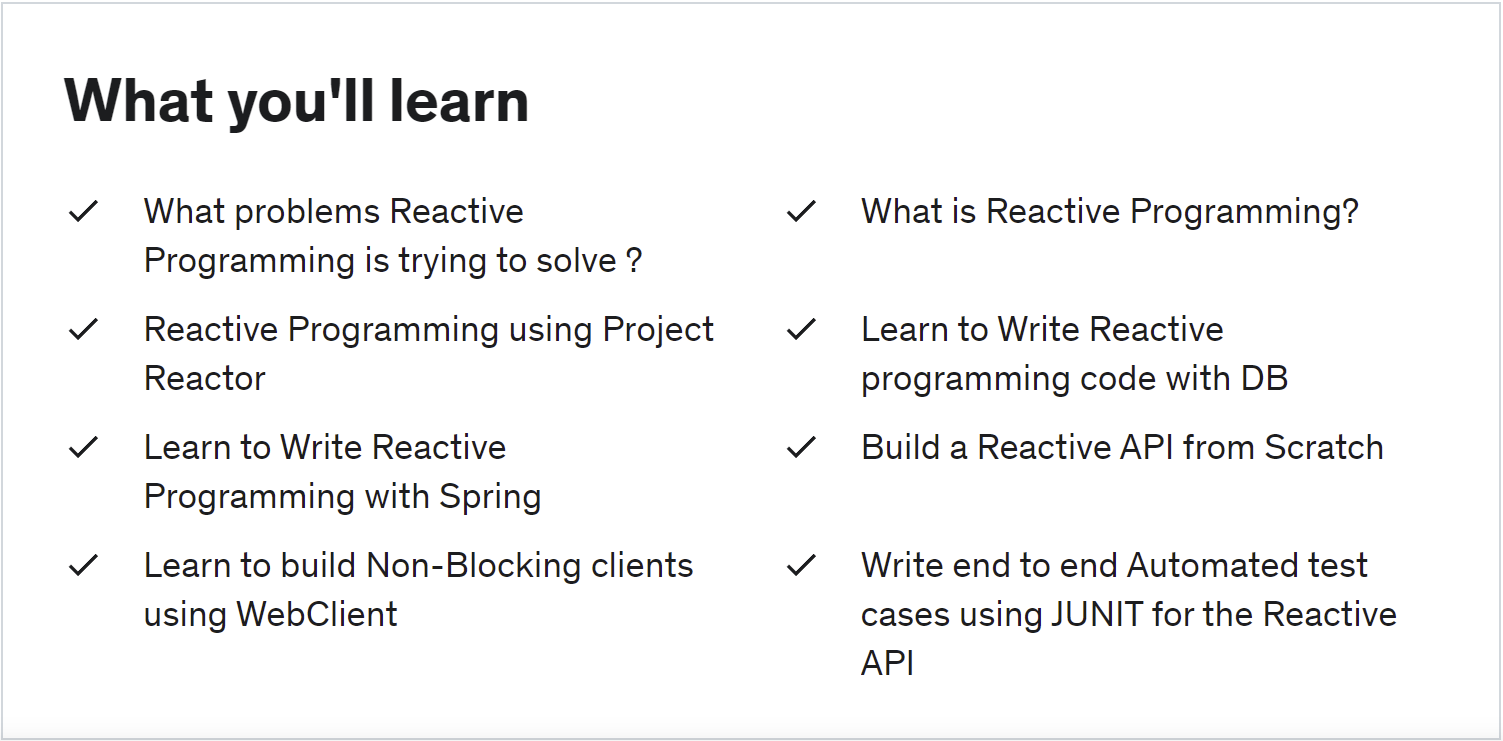
\includegraphics[width=14cm]{figuras/udemy1.png}
  \caption{Conteúdo do curso \textit{``Build Reactive MicroServices using Spring WebFlux/SpringBoot''} do \href{https://www.udemy.com/}{Udemy}}
  \label{fig:udemy1}
\end{figure}
\FloatBarrier

Seguidamente foi-me destacado o \href{https://www.udemy.com/course/grpc-the-complete-guide-for-java-developers/}{\textit{``Microservices with gRPC [Java + Spring Boot + Protobuf]''}}, que é um curso com o objetivo de ensinar ao estagiário a desenvolver \textit{microservices} com \href{https://grpc.io/}{gRPC} em \href{https://jdk.java.net/}{Java} usando \href{https://developers.google.com/protocol-buffers}{Protocol Buffers}, ou seja, um serviço que usa a implementação de RPC da \href{https://abc.xyz/}{Google} e usa o \href{https://developers.google.com/protocol-buffers}{Protocol Buffers} para o transporte de dados. Isto têm a vantagem de ser um serviço de baixo custo, e alta velocidade de comunicação.

\begin{figure}[!hbt]
  \centering
  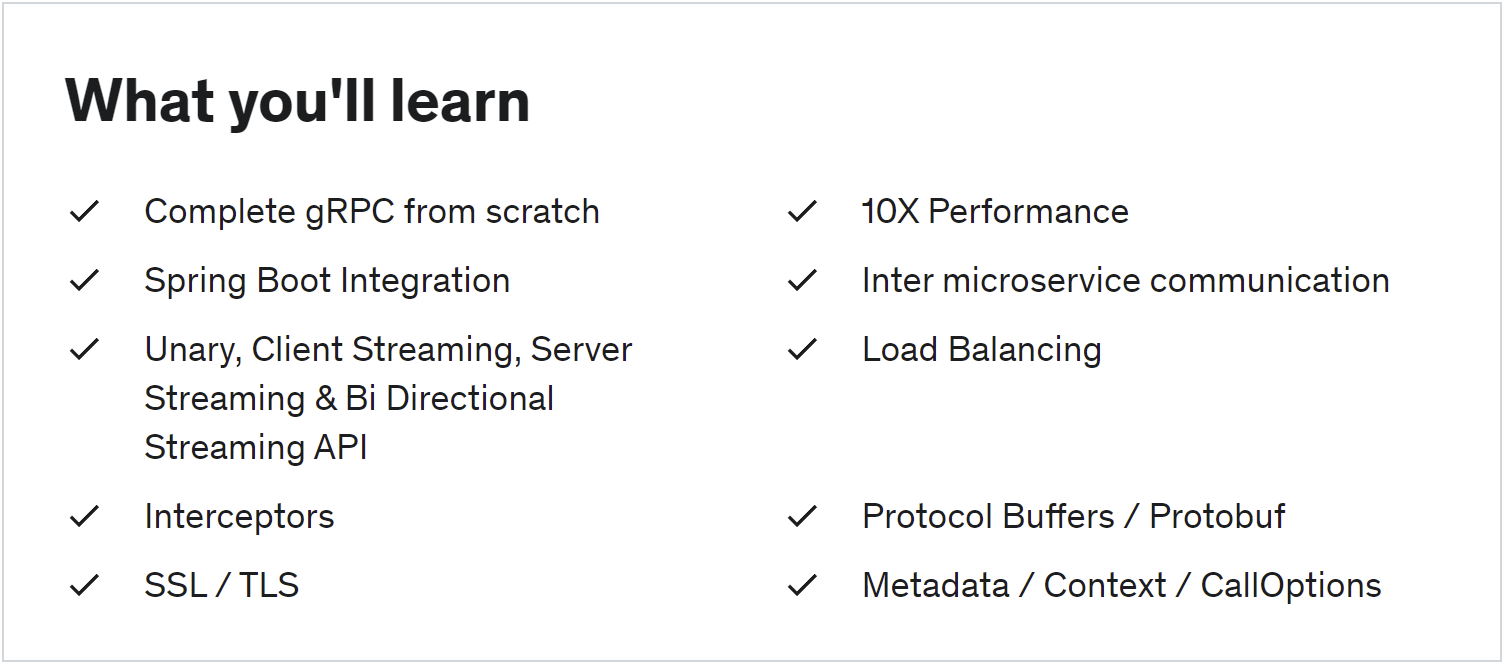
\includegraphics[width=14cm]{figuras/udemy2.png}
  \caption{Conteúdo do curso \textit{``Microservices with gRPC [Java + Spring Boot + Protobuf]''} do \href{https://www.udemy.com/}{Udemy}}
  \label{fig:udemy2}
\end{figure}
\FloatBarrier

O ultimo curso foi o \href{https://www.udemy.com/course/learn-micronaut/}{\textit{``Learn Micronaut - cloud native microservices with Java''}}, que nos mostra como fazer \textit{microservices} em Micronaut, um framework de \href{https://jdk.java.net/}{Java}, como o Spring mas com o objetivo de ser mais leve, modular e escalável. Este curso também passa pela integração do \href{https://kafka.apache.org/}{Apache Kafka}, um \textit{message broker} que permite a comunicação entre \textit{microservices} e como exportar o projeto para um \textit{native binary} e como usar o \href{https://www.graalvm.org/}{GraalVM}, que é uma JVM de nova geração, mais leve e mais rápida que também suporta outras linguagens de programação.

\begin{figure}[!hbt]
  \centering
  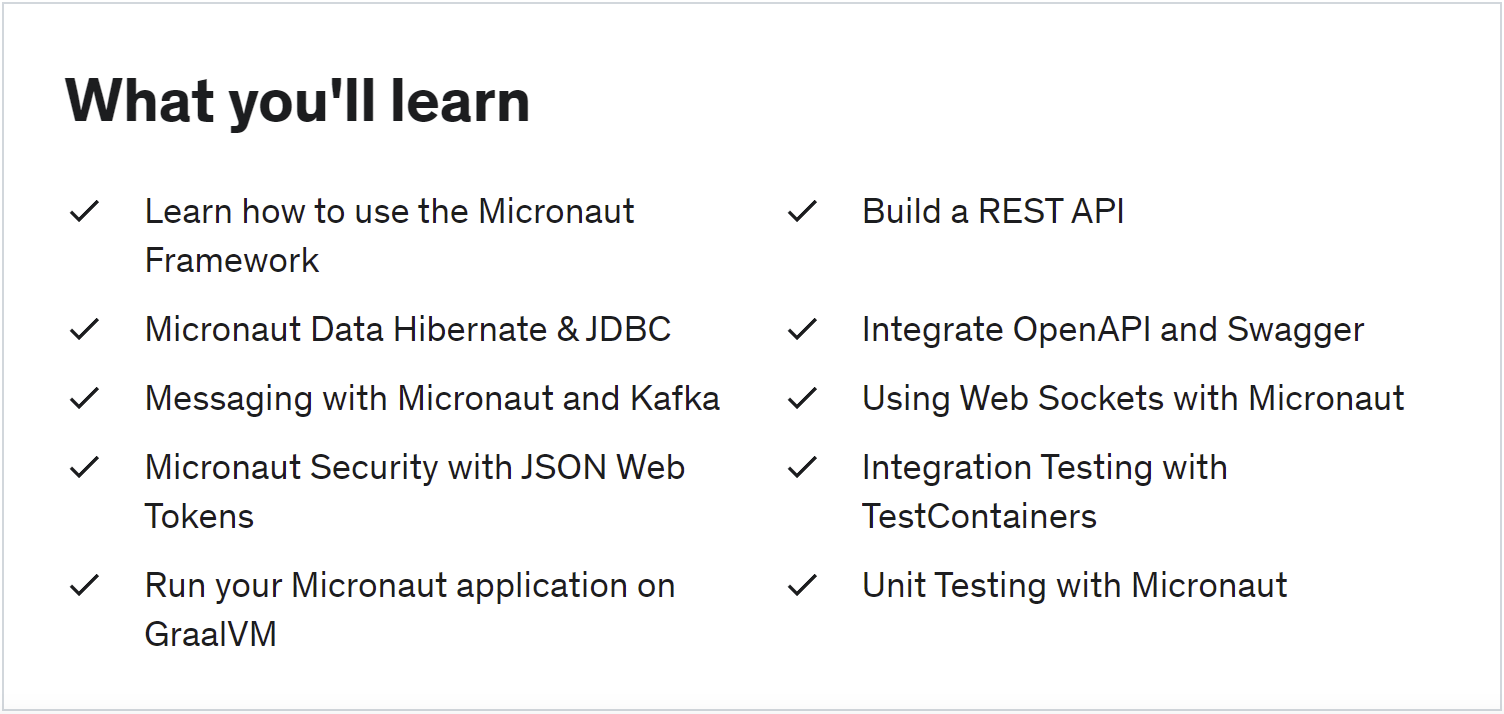
\includegraphics[width=14cm]{figuras/udemy3.png}
  \caption{Conteúdo do curso \textit{``Learn Micronaut - cloud native microservices with Java''} do \href{https://www.udemy.com/}{Udemy}}
  \label{fig:udemy3}
\end{figure}
\FloatBarrier

\chapter{Projeto}
\label{cap4}

Este capítulo descreve o projeto atribuído no estágio e o seu desenvolvimento. Sendo que este capítulo será o mais longo, mas consequentemente o mais importante e o mais complexo.

\section{Introdução}

Como anteriormente referido foi me destacada a tarefa de Implementação de um projeto no estágio. Este projeto consiste em um software que permite a gestão das especificações de Webshops.

Estas Webshops são, como o nome indica, as lojas online as quais são clientes da Optiply. Estas lojas online são responsáveis por fornecer os produtos que os clientes compram e a Optiply é responsável por fornecer a gestão inteligente dos produtos em stock.

O trabalho foi recebido num \textit{.pdf}, numa reunião de video-conferencia, com o coordenador do estágio (Fábio Belga), o seu subordinado (André Figueira)que ficou encarregado de orientar os estagiários de Backend, e nós (eu, Gonçalo Amaro e o estagiário da universade de Évora, José Azevedo), após a nossa fase formativa do \textit{Onboarding} descrita no capítulo anterior.

Assim, as primeiras secções deste capítulo servem como uma apresentação do equivalente à minha introdução ao projeto.

\section{Objetivos}

O objetivo descrito deste projeto é desenvolver um microserviço que permita a gestão das especificações de Webshops, já o verdadeiro objetivo deste projeto é fornecer treino ao estagiário nas tecnologias da \textit{Tech Stack} da empresa, ou pelo menos num dos projetos da mesma.

\newpage

Essa \textit{Tech Stack} referida é a seguinte:

\begin{itemize}
  \item Micronaut: Framework de desenvolvimento de microserviços.
  \item Java: Linguagem de programação.
  \item Gradle: Sistema de gestão de dependências e tarefas.
  \item jOOQ: Framework de código-fonte para acesso a bases de dados.
  \item Flyway: Framework de migração de bases de dados.
  \item PostgreSQL: Sistema de bases de dados.
  \item Junit5 (Spock também é aceitável): Framework de testes.
  \item Mockito: Framework de auxiliar a testes via simulação.
\end{itemize}

Voltando ao objetivo escrito do projeto (desenvolver um microserviço que permita a gestão das especificações de Webshops), o objetivo é desenvolver uma RESTful API que permita gerir as especificações de Webshops.

Para isso temos de saber que cada Webshop têm um conjunto de especificações, as quais são:

\begin{itemize}
  \item \textit{URL:} URL da loja online, têm validação e requer protocolo na URL;
  \item \textit{Handle:} identificador único da loja online;
  \item \textit{Interest Rate:} taxa de juros que a loja online paga, 20\% é o valor por defeito;
  \item \textit{Service Level Categories:} categorias de níveis de serviço que a loja têm, são três categorias (A,B e C) e as suas somas requerem ser iguais a 100\%;
  \item \textit{Contact Email List:} lista de emails de contacto da loja online, têm validação;
  \item \textbf{Extra:} \textit{Settings:} configurações da loja online:
        \begin{itemize}
          \item Enable Multi Supplier: permite múltiplos fornecedores;
          \item Enable Run Jobs: permite execução de tarefas;
          \item Currency: moeda da loja online em ISO-4217;
        \end{itemize}
\end{itemize}

Sendo que as ultimas especificações (as \textit{Settings}) são Extras, ou seja, não são obrigatórias, mas foram implementadas.
\newpage

Essa API tem um determinado conjunto de tarefas a cumprir as quais são:

\begin{itemize}
  \item Obter uma única Webshop;
  \item Obter várias Webshops:
        \begin{itemize}
          \item Deve ser capaz de ordenar e filtrar por qualquer campo da tabela;
          \item Só é necessário ordenar por um único campo. Os resultados devem ser consistentes com cada pedido. (Se ordenar por Taxa de Juros, como pode-se garantir que os mesmos resultados sejam obtidos em todos os pedidos?)
          \item Só é necessário filtrar por um único campo. Os filtros suportados são:
                \begin{itemize}
                  \item ``:'' significa \textbf{Igual}. Exemplo: handle:optiply 
                  \item ``\%'' significa \textbf{ILIKE} (semelhante, \textit{case-insensitive}). Exemplo: handle\%optiply
                  \item \textit{Extra:} ``>'' significa \textbf{Maior Que}. Exemplo: interestRate>20
                  \item \textit{Extra:} ``<'' significa \textbf{Menor Que}. Exemplo: interestRate<20
                \end{itemize}
        \end{itemize}
  \item Apagar uma única Webshop.
  \item Criar uma única Webshop.
  \item Atualizar qualquer campo da Webshop.
  \item \textit{Extra:} Filtrar por múltiplos campos.
  \item \textit{Extra:} Criar múltiplas Webshops.
  \item \textit{Extra:} Obter as configurações da Webshop.
  \item \textit{Extra:} Atualizar as configurações da Webshop.
\end{itemize}

Tendo sempre em conta que os resultados devem ser idempotentes e no seu estado mais recente e que os pedidos HTTP retornam:

\begin{itemize}
  \item Criar deve retornar 201.
  \item Obter e Atualizar devem retornar 200.
  \item Apagar deve retornar 204.
  \item Qualquer pedido deve retornar 404 se a loja não existir.
  \item Qualquer outro erro interno deve retornar 500 (Erro Interno).
\end{itemize}

Esta lista (tradução do que está no \textit{.pdf} recebido, que está também no \hyperref[ap1]{Apêndice I}), é bastante extensa, mas é bastante simples para entender o que é.

No entanto é estupidamente obscura a segunda intenção da lista, esta era a lista implícita de \textit{endpoints} da API. O qual inicialmente não vendo uma lista de \textit{endpoints} explicita nem uma mera referência na reunião, a primeira iteração do trabalho usei os \textit{endpoints} que eu achava mais convenientes para o trabalho. Escusado será dizer, que tive de os refazer após a primeira receção de \textit{feedback}.

\newpage

\section{Implementação}

\subsection{Inicio do Projecto}

\lipsum

\subsection{Metodologia de desenvolvimento}

\lipsum

\subsection{Testes}

\lipsum

\subsection{Feedback}

\lipsum

% para adicionar o  capítulo N adicione a linha \input{capituloN} e crie o ficheiro
% capituloN.tex na directoria "capitulos"

%%%%%%%%%%%%%%%%%%%%%%%%%%%%%%%%%%%%%%%%%%%%%%%%
% Bibliografia
\clearpage
\printbibliography[heading=bibintoc]
%%%%%%%%%%%%%%%%%%%%%%%%%%%%%%%%%%%%%%%%%%%%%%%%
\apendices
\chapter{Título do Apêndice I}
\label{ap1}

%a linha seguinte deve ser substituída pelo texto do apêndice
\lipsum
% para adicionar o  apêndice N adicione a linha \input{apendiceN} e crie o ficheiro
% apendiceN.tex na directoria "apendices"
%%%%%%%%%%%%%%%%%%%%%%%%%%%%%%%%%%%%%%%%%%%%%%%%
\anexos
\chapter{Implementação do \texttt{parseParamsWebshop}}\label{an1}

\lstinputlisting[frame=bt,language=java,caption={parseParamsWebshop()}]{listagens/parseParamsWebshop.java}
% para adicionar o  anexo N adicione a linha \input{anexoN} e crie o ficheiro
% anexoN.tex na directoria "anexos"
%%%%%%%%%%%%%%%%%%%%%%%%%%%%%%%%%%%%%%%%%%%%%%%%
\end{document}
